% Created 2012-05-25 Fri 12:20
\documentclass[compress, 9pt]{beamer}
\usepackage[utf8]{inputenc}
\usepackage[T1]{fontenc}
\usepackage{fixltx2e}
\usepackage{graphicx}
\usepackage{longtable}
\usepackage{float}
\usepackage{wrapfig}
\usepackage{soul}
\usepackage{textcomp}
\usepackage{marvosym}
\usepackage{wasysym}
\usepackage{latexsym}
\usepackage{amssymb}
\tolerance=1000
\usetheme{default}
\usecolortheme[RGB={0,38,93}]{structure}
\usefonttheme{serif}
\useinnertheme{circles}
\useoutertheme[]{shadow}
\setbeamertemplate{navigation symbols}{}
\usepackage{natbib}
\usepackage{fleqn}
\usepackage{epsf}
\usepackage[dvips]{color}
\usepackage{bibentry}
\institute{Computer Science and Engineering \\ University of Michigan}
\providecommand{\alert}[1]{\textbf{#1}}

\title{Probabilistic Inference}
\author{Shiwali Mohan}
\date{\today}
\hypersetup{
  pdfkeywords={},
  pdfsubject={},
  pdfcreator={Emacs Org-mode version 7.8.09}}

\begin{document}

\maketitle

\begin{frame}
\frametitle{Outline}
\setcounter{tocdepth}{3}
\tableofcontents
\end{frame}


\title[Search \hspace{1em}\insertframenumber/
\inserttotalframenumber]{Full Title}




\begin{frame}
\frametitle{Marginalization of Variables}
\label{sec-1}

\begin{figure}[htb]
\centering
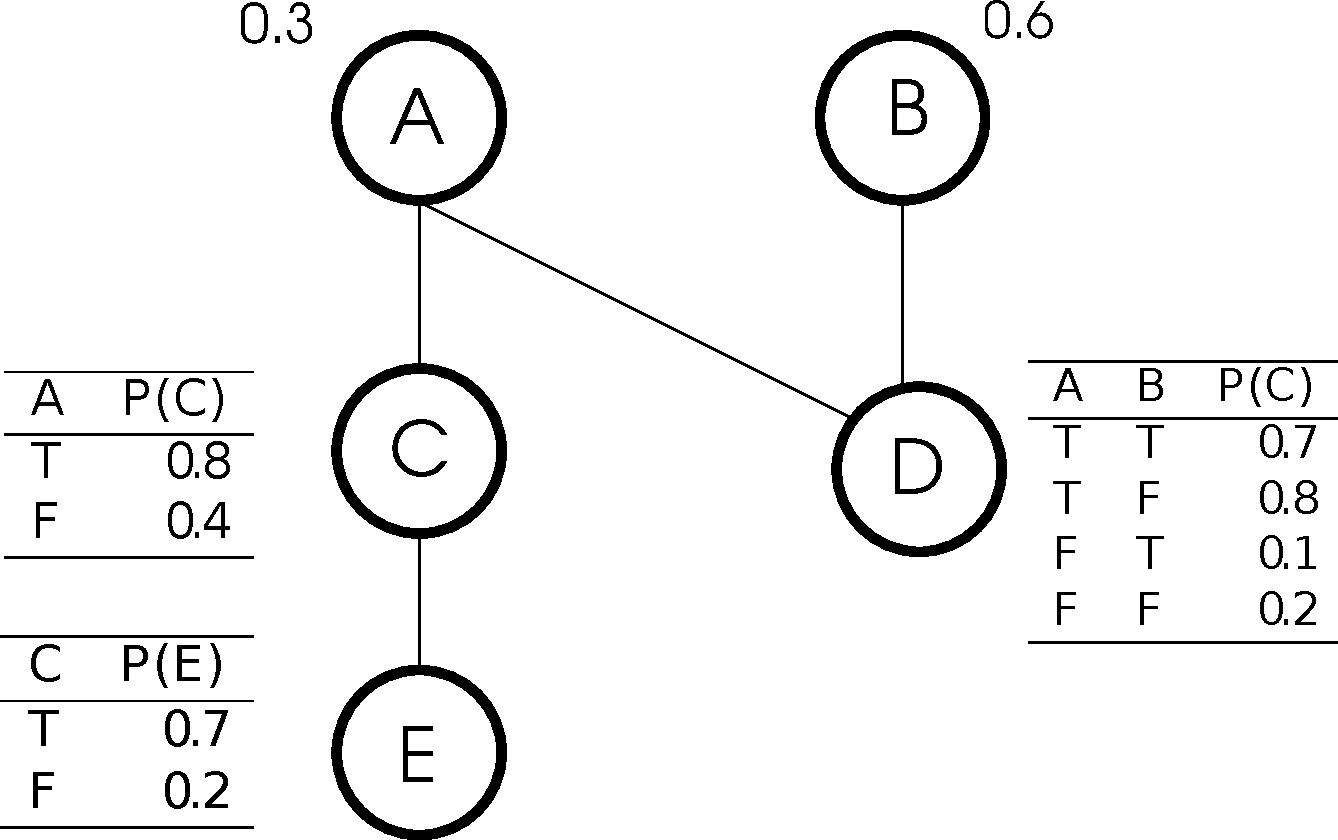
\includegraphics[width=8cm]{../images/bnet.pdf}
\caption{Bayes Net (A, B, C, D, E)}
\end{figure}
\begin{itemize}

\item Compute a CPT that gives probability of D in terms of B.
\label{sec-1-1}%
\begin{itemize}

\item <2-> B = T, P(C) = 0.7*0.3 + 0.1*0.7; B = F, P(C) = 0.8*0.3 + 0.2*0.7
\label{sec-1-1-1}%
\end{itemize} % ends low level

\item <3-> Compute a CPT that gives probability of E in term of A.
\label{sec-1-2}%
\begin{itemize}

\item <4-> A = T, P(E) = 0.8*0.7 + 0.2*0.2; A = F, P(E) = 0.4*0.7 + 0.6*0.2
\label{sec-1-2-1}%
\end{itemize} % ends low level
\end{itemize} % ends low level
\end{frame}
\begin{frame}
\frametitle{Utility of an action}
\label{sec-2}

Two banks are on the x axis. Left-bank is at lbx=0 and right-bank is
at rbx=20. Agent's location on the number line is at 0<a<20. The agent
has 5\$. If it goes to left-bank, it can get 20\$. If it goes to the
right-bank, it can get 10\$. However, in order to get to the bank the
agent has to spend money at the rate of 2*(distance from the
bank). The agent has three actions - go-left, go-right and stay. The
agent wants to maximize the money it has. Left-bank might be closed with a probability
of 0.25, right-bank might be closed with a probability of 0.20. 
\begin{itemize}

\item <1-> What is the expected utility of each action for a position x?
\label{sec-2-1}%
\begin{itemize}

\item <2-> EU(stay) = 5\\
\label{sec-2-1-1}%
EU(go-left) = 5 + (0.75*20 + 0.25*0) - 2*x\\
     EU(go-right) = 5 + (0.80*10 + 0.20*0) - 2(20-x)
\end{itemize} % ends low level

\item <3-> What are the threshold (in terms of distances) for optimal action?
\label{sec-2-2}%
\begin{itemize}

\item <4-> threshold 7.5-16
\label{sec-2-2-1}%
\end{itemize} % ends low level
\end{itemize} % ends low level
\end{frame}
\begin{frame}
\frametitle{JavaBayes Demo}
\label{sec-3}
\end{frame}

\end{document}
